

\documentclass[preview,border=4mm,convert={density=600,outext=.png}]{standalone}

\usepackage{url}
\usepackage{tikz}
\usepackage{color}
\begin{document}

\tikzset{every picture/.style={line width=0.75pt}} %set default line width to 0.75pt

\begin{tikzpicture}[x=0.75pt,y=0.75pt,yscale=-1,xscale=1]
%uncomment if require: \path (0,300); %set diagram left start at 0, and has height of 300

%Rounded Rect [id:dp6996926995502989]
\draw   (86,94.6) .. controls (86,87.09) and (92.09,81) .. (99.6,81) -- (317.4,81) .. controls (324.91,81) and (331,87.09) .. (331,94.6) -- (331,135.4) .. controls (331,142.91) and (324.91,149) .. (317.4,149) -- (99.6,149) .. controls (92.09,149) and (86,142.91) .. (86,135.4) -- cycle ;
%Image [id:dp5199524107849971]
\draw (302.2,113.2) node  {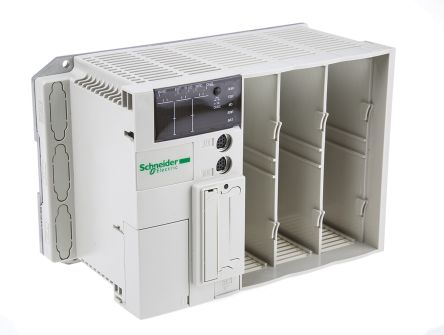
\includegraphics[width=43.2pt,height=43.2pt]{images/automate_schneider.jpg}};
%Rounded Rect [id:dp4357143022979344]
\draw  [fill={rgb, 255:red, 255; green, 245; blue, 245 }  ,fill opacity=1 ][line width=0.75]  (20.83,194.2) .. controls (20.83,181.39) and (31.21,171) .. (44.03,171) -- (372.97,171) .. controls (385.79,171) and (396.17,181.39) .. (396.17,194.2) -- (396.17,263.8) .. controls (396.17,276.61) and (385.79,287) .. (372.97,287) -- (44.03,287) .. controls (31.21,287) and (20.83,276.61) .. (20.83,263.8) -- cycle ;
%Rounded Rect [id:dp8390570092351776]
\draw  [color={rgb, 255:red, 208; green, 2; blue, 27 }  ,draw opacity=1 ][line width=1.5]  (40,189) .. controls (40,184.58) and (43.58,181) .. (48,181) -- (102,181) .. controls (106.42,181) and (110,184.58) .. (110,189) -- (110,213) .. controls (110,217.42) and (106.42,221) .. (102,221) -- (48,221) .. controls (43.58,221) and (40,217.42) .. (40,213) -- cycle ;
%Rounded Rect [id:dp9242421121217611]
\draw  [color={rgb, 255:red, 65; green, 117; blue, 5 }  ,draw opacity=1 ][line width=1.5]  (274,191) .. controls (274,186.58) and (277.58,183) .. (282,183) -- (380,183) .. controls (384.42,183) and (388,186.58) .. (388,191) -- (388,215) .. controls (388,219.42) and (384.42,223) .. (380,223) -- (282,223) .. controls (277.58,223) and (274,219.42) .. (274,215) -- cycle ;
%Rounded Rect [id:dp5921159806431459]
\draw  [line width=0.75]  (157,229) .. controls (157,224.58) and (160.58,221) .. (165,221) -- (252,221) .. controls (256.42,221) and (260,224.58) .. (260,229) -- (260,253) .. controls (260,257.42) and (256.42,261) .. (252,261) -- (165,261) .. controls (160.58,261) and (157,257.42) .. (157,253) -- cycle ;

%Curve Lines [id:da49513234525320104]
\draw [color={rgb, 255:red, 208; green, 2; blue, 27 }  ,draw opacity=1 ]   (48,181) .. controls (43.13,107.87) and (62.97,116.5) .. (85.28,116.05) ;
\draw [shift={(87,116)}, rotate = 537.51] [color={rgb, 255:red, 208; green, 2; blue, 27 }  ,draw opacity=1 ][line width=0.75]    (10.93,-3.29) .. controls (6.95,-1.4) and (3.31,-0.3) .. (0,0) .. controls (3.31,0.3) and (6.95,1.4) .. (10.93,3.29)   ;

%Curve Lines [id:da8679026938428056]
\draw [color={rgb, 255:red, 65; green, 117; blue, 5 }  ,draw opacity=1 ]   (331,112) .. controls (387.43,107.05) and (351.73,129.54) .. (352.95,180.45) ;
\draw [shift={(353,182)}, rotate = 267.8] [color={rgb, 255:red, 65; green, 117; blue, 5 }  ,draw opacity=1 ][line width=0.75]    (10.93,-3.29) .. controls (6.95,-1.4) and (3.31,-0.3) .. (0,0) .. controls (3.31,0.3) and (6.95,1.4) .. (10.93,3.29)   ;

%Curve Lines [id:da11237972281185649]
\draw    (335,223) .. controls (334.01,240.82) and (318.32,243.94) .. (264.64,241.09) ;
\draw [shift={(263,241)}, rotate = 363.12] [color={rgb, 255:red, 0; green, 0; blue, 0 }  ][line width=0.75]    (10.93,-3.29) .. controls (6.95,-1.4) and (3.31,-0.3) .. (0,0) .. controls (3.31,0.3) and (6.95,1.4) .. (10.93,3.29)   ;

%Curve Lines [id:da3503728176891857]
\draw    (157,243) .. controls (61.94,241.04) and (71.56,253.49) .. (71.99,223.87) ;
\draw [shift={(72,222)}, rotate = 450] [color={rgb, 255:red, 0; green, 0; blue, 0 }  ][line width=0.75]    (10.93,-3.29) .. controls (6.95,-1.4) and (3.31,-0.3) .. (0,0) .. controls (3.31,0.3) and (6.95,1.4) .. (10.93,3.29)   ;

%Straight Lines [id:da7532920416250504]
\draw [color={rgb, 255:red, 208; green, 2; blue, 27 }  ,draw opacity=1 ]   (159,80) -- (159,39) ;
\draw [shift={(159,37)}, rotate = 450] [color={rgb, 255:red, 208; green, 2; blue, 27 }  ,draw opacity=1 ][line width=0.75]    (10.93,-3.29) .. controls (6.95,-1.4) and (3.31,-0.3) .. (0,0) .. controls (3.31,0.3) and (6.95,1.4) .. (10.93,3.29)   ;

%Straight Lines [id:da741979851639265]
\draw [color={rgb, 255:red, 74; green, 144; blue, 226 }  ,draw opacity=1 ]   (141,51) -- (141,77) ;
\draw [shift={(141,79)}, rotate = 270] [color={rgb, 255:red, 74; green, 144; blue, 226 }  ,draw opacity=1 ][line width=0.75]    (10.93,-3.29) .. controls (6.95,-1.4) and (3.31,-0.3) .. (0,0) .. controls (3.31,0.3) and (6.95,1.4) .. (10.93,3.29)   ;

%Rounded Rect [id:dp2079891174972378]
\draw  [dash pattern={on 4.5pt off 4.5pt}] (102,27.4) .. controls (102,23.31) and (105.31,20) .. (109.4,20) -- (194.6,20) .. controls (198.69,20) and (202,23.31) .. (202,27.4) -- (202,49.6) .. controls (202,53.69) and (198.69,57) .. (194.6,57) -- (109.4,57) .. controls (105.31,57) and (102,53.69) .. (102,49.6) -- cycle ;
%Rounded Rect [id:dp14823711603822332]
\draw  [dash pattern={on 4.5pt off 4.5pt}] (245,30) .. controls (245,25.58) and (248.58,22) .. (253,22) -- (307,22) .. controls (311.42,22) and (315,25.58) .. (315,30) -- (315,54) .. controls (315,58.42) and (311.42,62) .. (307,62) -- (253,62) .. controls (248.58,62) and (245,58.42) .. (245,54) -- cycle ;

% Text Node
\draw (208.5,276) node [scale=0.9] [align=left] {Partie opérative};
% Text Node
\draw (75,201) node [color={rgb, 255:red, 208; green, 2; blue, 27 }  ,opacity=1 ] [align=left] {Capteurs};
% Text Node
\draw (332,202) node [color={rgb, 255:red, 65; green, 117; blue, 5 }  ,opacity=1 ] [align=left] {Pré-actionneurs};
% Text Node
\draw (209.5,136) node [scale=0.9] [align=left] {Partie commande};
% Text Node
\draw (384,102) node [color={rgb, 255:red, 65; green, 117; blue, 5 }  ,opacity=1 ] [align=left] {commandes};
% Text Node
\draw (43,106) node [color={rgb, 255:red, 208; green, 2; blue, 27 }  ,opacity=1 ] [align=left] {Informations};
% Text Node
\draw (126,43) node [color={rgb, 255:red, 74; green, 144; blue, 226 }  ,opacity=1 ] [align=left] {{\footnotesize ordres}};
% Text Node
\draw (154,29) node [color={rgb, 255:red, 208; green, 2; blue, 27 }  ,opacity=1 ] [align=left] {{\footnotesize Informations}};
% Text Node
\draw (182,47) node [scale=0.9] [align=left] {IHM};
% Text Node
\draw (186,110) node  [align=left] {Automate Programmable};
% Text Node
\draw (280,52) node [scale=0.9] [align=left] {Réseau};
% Text Node
\draw (209,240) node  [align=left] {Actionneurs};


\end{tikzpicture}


\end{document}
